\section{Preliminary Evaluation}
\label{sec:eval}

% \begin{itemize}
%   \item Experiment on datas from the Bureau of Transportation Statistic (\url{http://www.transtats.bts.gov/Fields.asp?Table_ID=236}) to evaluate flight delays by airport
%   \item Infrastructure based on ONE cluster, VM 16.04 LTS (GNU/Linux 4.4.0-53-generic x86\_64), Docker 1.13.0-rc3, Docker Swarm 1.2.5 (discovery: Consul v0.5.2)
%   \item Hardware?
% \end{itemize}
This section presents our preliminary evaluation of \SYS.
First we present our evaluation settings, then the dataset and finally some preliminary benchmark, namely in terms of throughput and scalability.

\textbf{Evaluation settings.} We use a cluster of virtual machines based on Ubuntu 16.04 LTS OS and running a daemon Docker 1.13.0-rc3.
Each VM is set with 2 CPU cores and 2GB RAM.
Nodes are clusterised by Docker Swarm 1.2.5, using Consul 0.5.2 as discovery service.
A single-one container is launch on each node.
Containers are communicating accross a Docker overlay network.

\textbf{Dataset.} In our experiments we process a real dataset released by the American Bureau of Transportation Statistic\cite{rita:bts}, including each flight's departure and arrivals\cite{statistical_computing:data}.
The dataset reports the flight departures and arrivals of 20 air carriers.\ah{pointers on datas are not relevant?}
We implement a simple application on top of \SYS to determine average delays and the total of delayed flights for each air carrier.
%These datas report flights departures and arrivals\cite{rita:bts} and are available on the Statistical Computing\cite{statistical_computing:data}.
We design and implement a simple processing pipeline, that (i) parses the input datasets (in a comma-separated-value format) to data structure (map), (ii) filters by relevancy (i.e. if the data concerns a delayed flight), and (iii) finally reduces to compute the wanted insights.\footnote{This experiment is inspired by the blog post \emph{Diving into Akka Streams} written by Kevin Webber (\url{https://blog.redelastic.com/diving-into-akka-streams-2770b3aeabb0})}
We use the 4 last years of the available dataset (from 2005 to 2008), for a total of 28 millions of entries to process.


\textbf{Benchmark: throughput}
\ah{expose throughput results}
Throughput accross containers wrapping each node of the processing pipeline are measured from Docker stats.
During the experiment, we retrieve all the data stats for each container.
In particular, \texttt{txbytes} stats are extracted to measure containers output throughput.
These datas are computed to be plotted together by percentile, as shown on figure \ref{fig:throughput}.\ah{maybe it could be relevant to put three plots, corresponding to experiments 4-datas-1-worker, 4-datas-2-workers and 4-datas-4-workers}
A maximum of around 10MB/s throughput between containers then is observed.\ah{I gonna measure throuput between two containers run on a swarm cluster, using iperf, for comparison purpose}


\begin{figure}[t!]
  \centering
  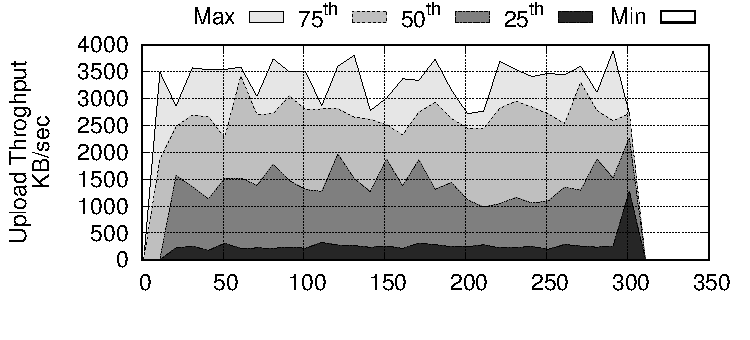
\includegraphics[width=.99\linewidth]{images/tput_upload}
  \caption{Throughput.}
  \label{fig:throughput}
\end{figure}

\textbf{Benchmark: scalability}
Scalability of \SYS is evaluated by processing these datas 20 times on 3 different pipeline topology: using 1, 2 or 4 workers for each step of the pipeline.
Results are represented on figure \ref{fig:scalability}, and show clearly better performances between the experiment using only one worker by task, and the one using 2 workers.
In an other hand, using 4 workers instead of 2 does not show any performance improvement.

\begin{figure}[t!]
  \centering
  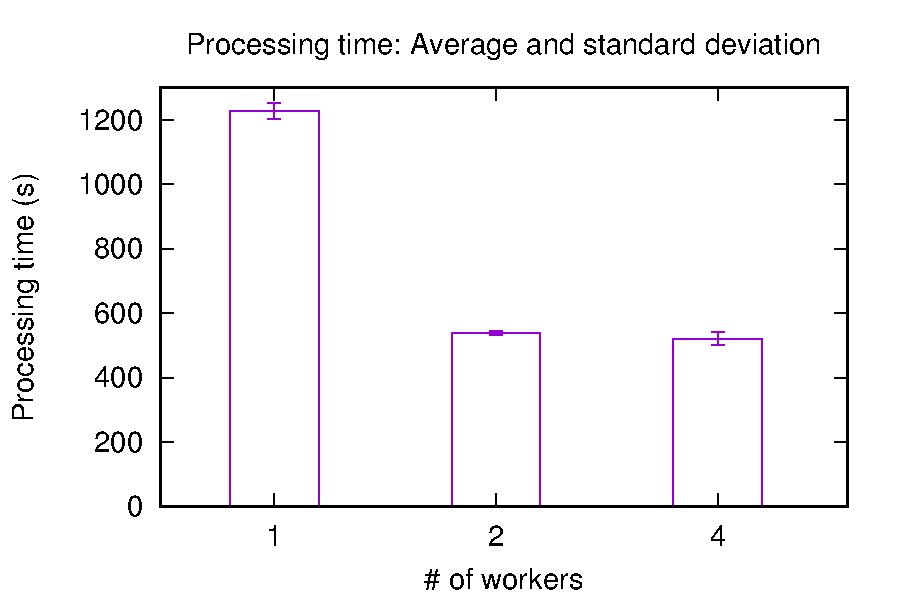
\includegraphics[width=.99\linewidth]{images/avg_stdev_4_streams}
  \caption{Scalability.}
  \label{fig:scalability}
\end{figure}

The latter observation can be explained by the fact that each job in our experiment is very simple and executed too quickly by the workers, compared to the throughput capacity of the communication between two steps of the process pipeline.
This may be due to the limitation of the network bandwith capacity, when the cost of data communication accross nodes is higher than the one of data computation, as described by the Gunther's Universal Law of Computational Scalability\cite{gunther1993simple}, where the relative capacity of a computational platform is inversely proportional to the sum of the levels of contention (e.g., queueing for shared resources) and coherency delay (i.e., latency for data to become consistent) in the system.
In an other hand, it may also be due to the limitation of the router bandwith, the improvement of which is a part of our future work.
